% Options for packages loaded elsewhere
\PassOptionsToPackage{unicode}{hyperref}
\PassOptionsToPackage{hyphens}{url}
%
\documentclass[
]{article}
\usepackage{amsmath,amssymb}
\usepackage{iftex}
\ifPDFTeX
  \usepackage[T1]{fontenc}
  \usepackage[utf8]{inputenc}
  \usepackage{textcomp} % provide euro and other symbols
\else % if luatex or xetex
  \usepackage{unicode-math} % this also loads fontspec
  \defaultfontfeatures{Scale=MatchLowercase}
  \defaultfontfeatures[\rmfamily]{Ligatures=TeX,Scale=1}
\fi
\usepackage{lmodern}
\ifPDFTeX\else
  % xetex/luatex font selection
\fi
% Use upquote if available, for straight quotes in verbatim environments
\IfFileExists{upquote.sty}{\usepackage{upquote}}{}
\IfFileExists{microtype.sty}{% use microtype if available
  \usepackage[]{microtype}
  \UseMicrotypeSet[protrusion]{basicmath} % disable protrusion for tt fonts
}{}
\makeatletter
\@ifundefined{KOMAClassName}{% if non-KOMA class
  \IfFileExists{parskip.sty}{%
    \usepackage{parskip}
  }{% else
    \setlength{\parindent}{0pt}
    \setlength{\parskip}{6pt plus 2pt minus 1pt}}
}{% if KOMA class
  \KOMAoptions{parskip=half}}
\makeatother
\usepackage{xcolor}
\usepackage[margin=1in]{geometry}
\usepackage{color}
\usepackage{fancyvrb}
\newcommand{\VerbBar}{|}
\newcommand{\VERB}{\Verb[commandchars=\\\{\}]}
\DefineVerbatimEnvironment{Highlighting}{Verbatim}{commandchars=\\\{\}}
% Add ',fontsize=\small' for more characters per line
\usepackage{framed}
\definecolor{shadecolor}{RGB}{248,248,248}
\newenvironment{Shaded}{\begin{snugshade}}{\end{snugshade}}
\newcommand{\AlertTok}[1]{\textcolor[rgb]{0.94,0.16,0.16}{#1}}
\newcommand{\AnnotationTok}[1]{\textcolor[rgb]{0.56,0.35,0.01}{\textbf{\textit{#1}}}}
\newcommand{\AttributeTok}[1]{\textcolor[rgb]{0.13,0.29,0.53}{#1}}
\newcommand{\BaseNTok}[1]{\textcolor[rgb]{0.00,0.00,0.81}{#1}}
\newcommand{\BuiltInTok}[1]{#1}
\newcommand{\CharTok}[1]{\textcolor[rgb]{0.31,0.60,0.02}{#1}}
\newcommand{\CommentTok}[1]{\textcolor[rgb]{0.56,0.35,0.01}{\textit{#1}}}
\newcommand{\CommentVarTok}[1]{\textcolor[rgb]{0.56,0.35,0.01}{\textbf{\textit{#1}}}}
\newcommand{\ConstantTok}[1]{\textcolor[rgb]{0.56,0.35,0.01}{#1}}
\newcommand{\ControlFlowTok}[1]{\textcolor[rgb]{0.13,0.29,0.53}{\textbf{#1}}}
\newcommand{\DataTypeTok}[1]{\textcolor[rgb]{0.13,0.29,0.53}{#1}}
\newcommand{\DecValTok}[1]{\textcolor[rgb]{0.00,0.00,0.81}{#1}}
\newcommand{\DocumentationTok}[1]{\textcolor[rgb]{0.56,0.35,0.01}{\textbf{\textit{#1}}}}
\newcommand{\ErrorTok}[1]{\textcolor[rgb]{0.64,0.00,0.00}{\textbf{#1}}}
\newcommand{\ExtensionTok}[1]{#1}
\newcommand{\FloatTok}[1]{\textcolor[rgb]{0.00,0.00,0.81}{#1}}
\newcommand{\FunctionTok}[1]{\textcolor[rgb]{0.13,0.29,0.53}{\textbf{#1}}}
\newcommand{\ImportTok}[1]{#1}
\newcommand{\InformationTok}[1]{\textcolor[rgb]{0.56,0.35,0.01}{\textbf{\textit{#1}}}}
\newcommand{\KeywordTok}[1]{\textcolor[rgb]{0.13,0.29,0.53}{\textbf{#1}}}
\newcommand{\NormalTok}[1]{#1}
\newcommand{\OperatorTok}[1]{\textcolor[rgb]{0.81,0.36,0.00}{\textbf{#1}}}
\newcommand{\OtherTok}[1]{\textcolor[rgb]{0.56,0.35,0.01}{#1}}
\newcommand{\PreprocessorTok}[1]{\textcolor[rgb]{0.56,0.35,0.01}{\textit{#1}}}
\newcommand{\RegionMarkerTok}[1]{#1}
\newcommand{\SpecialCharTok}[1]{\textcolor[rgb]{0.81,0.36,0.00}{\textbf{#1}}}
\newcommand{\SpecialStringTok}[1]{\textcolor[rgb]{0.31,0.60,0.02}{#1}}
\newcommand{\StringTok}[1]{\textcolor[rgb]{0.31,0.60,0.02}{#1}}
\newcommand{\VariableTok}[1]{\textcolor[rgb]{0.00,0.00,0.00}{#1}}
\newcommand{\VerbatimStringTok}[1]{\textcolor[rgb]{0.31,0.60,0.02}{#1}}
\newcommand{\WarningTok}[1]{\textcolor[rgb]{0.56,0.35,0.01}{\textbf{\textit{#1}}}}
\usepackage{graphicx}
\makeatletter
\def\maxwidth{\ifdim\Gin@nat@width>\linewidth\linewidth\else\Gin@nat@width\fi}
\def\maxheight{\ifdim\Gin@nat@height>\textheight\textheight\else\Gin@nat@height\fi}
\makeatother
% Scale images if necessary, so that they will not overflow the page
% margins by default, and it is still possible to overwrite the defaults
% using explicit options in \includegraphics[width, height, ...]{}
\setkeys{Gin}{width=\maxwidth,height=\maxheight,keepaspectratio}
% Set default figure placement to htbp
\makeatletter
\def\fps@figure{htbp}
\makeatother
\setlength{\emergencystretch}{3em} % prevent overfull lines
\providecommand{\tightlist}{%
  \setlength{\itemsep}{0pt}\setlength{\parskip}{0pt}}
\setcounter{secnumdepth}{-\maxdimen} % remove section numbering
\usepackage{booktabs}
\usepackage{longtable}
\usepackage{array}
\usepackage{multirow}
\usepackage{wrapfig}
\usepackage{float}
\usepackage{colortbl}
\usepackage{pdflscape}
\usepackage{tabu}
\usepackage{threeparttable}
\usepackage{threeparttablex}
\usepackage[normalem]{ulem}
\usepackage{makecell}
\usepackage{xcolor}
\ifLuaTeX
  \usepackage{selnolig}  % disable illegal ligatures
\fi
\usepackage{bookmark}
\IfFileExists{xurl.sty}{\usepackage{xurl}}{} % add URL line breaks if available
\urlstyle{same}
\hypersetup{
  hidelinks,
  pdfcreator={LaTeX via pandoc}}

\author{}
\date{\vspace{-2.5em}}

\begin{document}

\newpage
\begin{titlepage}
\begin{center}

\large
UNIVERSIDADE FEDERAL DE UBERLÂNDIA\\
FACULDADE DE ENGENHARIA ELÉTRICA\\
GRADUAÇÃO EM ENGENHARIA BIOMÉDICA\\[7cm]

\Large
\textbf{Heitor Pereira Nunes Fernandes Cunha}\\[2cm]

\textbf{\large Processamento de Sinais Biomédicos: Módulo 4}\\[10cm]

\large
Uberlândia, MG\\
2025

\end{center}
\end{titlepage}

\newpage
\section*{Questão 1}

\begin{quote}
A avaliação de estatísticas de um sinal biomédico é de grande relevância
para a caracterização do sinal e para o desenvolvimento de dispositivos.
Por exemplo, ao monitorarmos a atividade eletromiográfica ao longo do
tempo e estimarmos estatísticas (e.g., a média do valor absoluto) do
sinal é possível realizar o controle de dispositivos miolétricos. De
forma genérica, o sinal eletromiográfico pode ser simulado a partir de
amostras de uma distribuição normal, que possui uma média zero e desvio
padrão unitário. Considerando essas informações você deve:
\end{quote}

\begin{quote}
Simular um sinal eletromiográfico, EMG1, amostrado a 1000 Hz, de
duração, t, de 30 segundos, cuja a média é 0.8 e o devio padrão é 1.3.
Deve-se plotar o gráfico mostrando o sinal gerado.
\end{quote}

\begin{Shaded}
\begin{Highlighting}[]
\FunctionTok{library}\NormalTok{(pracma)}
\FunctionTok{library}\NormalTok{(tidyverse)}
\end{Highlighting}
\end{Shaded}

\begin{verbatim}
## -- Attaching core tidyverse packages ------------------------ tidyverse 2.0.0 --
## v dplyr     1.1.4     v readr     2.1.5
## v forcats   1.0.0     v stringr   1.5.1
## v ggplot2   3.5.1     v tibble    3.2.1
## v lubridate 1.9.4     v tidyr     1.3.1
## v purrr     1.0.4     
## -- Conflicts ------------------------------------------ tidyverse_conflicts() --
## x purrr::cross()  masks pracma::cross()
## x dplyr::filter() masks stats::filter()
## x dplyr::lag()    masks stats::lag()
## i Use the conflicted package (<http://conflicted.r-lib.org/>) to force all conflicts to become errors
\end{verbatim}

\begin{Shaded}
\begin{Highlighting}[]
\CommentTok{\# Frequência de amostragem}
\NormalTok{fs }\OtherTok{\textless{}{-}} \DecValTok{1000}

\NormalTok{dt }\OtherTok{\textless{}{-}} \DecValTok{1}\SpecialCharTok{/}\NormalTok{fs}

\CommentTok{\# Vetor de tempo "t"}
\NormalTok{t }\OtherTok{\textless{}{-}} \FunctionTok{seq}\NormalTok{(}\AttributeTok{from =} \DecValTok{0}\NormalTok{, }\AttributeTok{to =} \DecValTok{30}\NormalTok{, }\AttributeTok{by =}\NormalTok{ dt)}

\CommentTok{\# Média desejada}
\NormalTok{media }\OtherTok{\textless{}{-}} \FloatTok{0.8}

\CommentTok{\# Desvio padrão desejado}
\NormalTok{desvio\_padrao }\OtherTok{\textless{}{-}} \FloatTok{1.3}

\CommentTok{\# Numero de amostrar}
\NormalTok{amostras }\OtherTok{\textless{}{-}}\NormalTok{ fs }\SpecialCharTok{*}\NormalTok{ t}

\CommentTok{\# Calculando amplitudes do EMG1 com base na funcao randn()}
\NormalTok{amplitudes\_ }\OtherTok{\textless{}{-}} \FunctionTok{randn}\NormalTok{(}\AttributeTok{n =} \FunctionTok{length}\NormalTok{(t), }\AttributeTok{m =} \DecValTok{1}\NormalTok{)}

\NormalTok{amplitudes\_EMG1 }\OtherTok{\textless{}{-}}\NormalTok{ media }\SpecialCharTok{+}\NormalTok{ desvio\_padrao }\SpecialCharTok{*}\NormalTok{ amplitudes\_}

\CommentTok{\# Criando um dataframe para o sinal EMG1}

\NormalTok{df\_EMG1 }\OtherTok{\textless{}{-}} \FunctionTok{data.frame}\NormalTok{(}\AttributeTok{Amplitudes =}\NormalTok{ amplitudes\_EMG1, }\AttributeTok{t =}\NormalTok{ t)}

\CommentTok{\# Plotando o sinal EMG1 com o ggplot}

\NormalTok{ggplot\_1 }\OtherTok{\textless{}{-}}\NormalTok{ ggplot2}\SpecialCharTok{::}\FunctionTok{ggplot}\NormalTok{(df\_EMG1, }\FunctionTok{aes}\NormalTok{ (}\AttributeTok{x =}\NormalTok{ t, }\AttributeTok{y =}\NormalTok{ Amplitudes)) }\SpecialCharTok{+}
  \FunctionTok{geom\_line}\NormalTok{() }\SpecialCharTok{+}
  \FunctionTok{xlab}\NormalTok{(}\StringTok{"Tempo (s)"}\NormalTok{) }\SpecialCharTok{+}
  \FunctionTok{ylab}\NormalTok{(}\StringTok{"EMG1 simulado"}\NormalTok{)}

\NormalTok{ggplot\_1}
\end{Highlighting}
\end{Shaded}

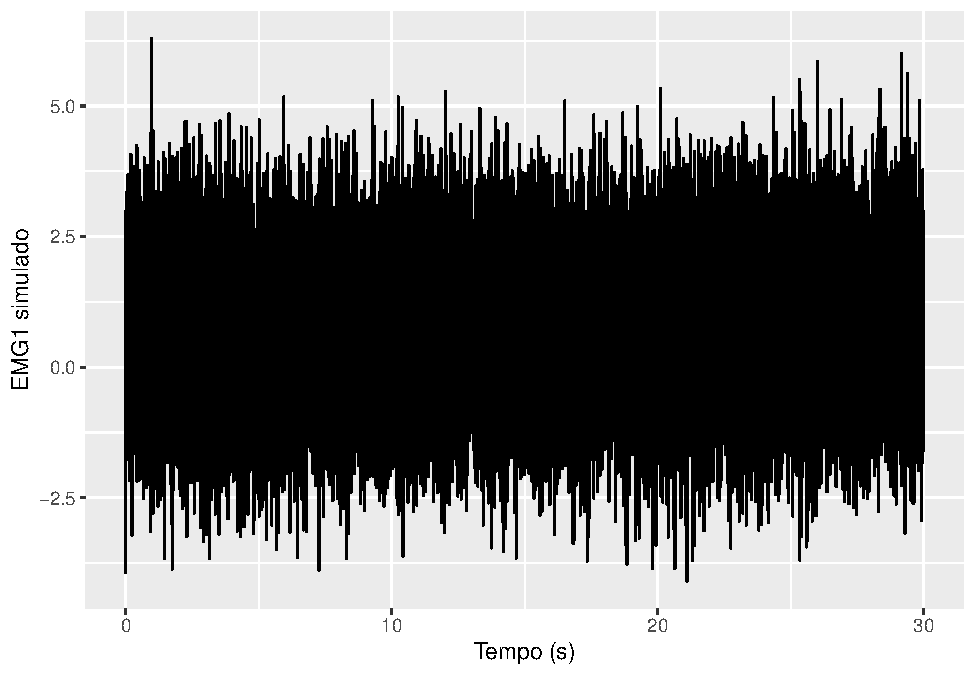
\includegraphics{Modulo4_files/figure-latex/unnamed-chunk-1-1.pdf}

\begin{quote}
Simular um sinal eletromiográfico, EMG2, amostrado a 300 Hz, de duração,
t, de 30 segundos, cuja a média é 1.8 e o devio padrão é 0.9. Deve-se
plotar o gráfico mostrando o sinal gerado.
\end{quote}

\begin{Shaded}
\begin{Highlighting}[]
\FunctionTok{library}\NormalTok{(pracma)}
\FunctionTok{library}\NormalTok{(tidyverse)}

\CommentTok{\# Frequência de amostragem}
\NormalTok{fs2 }\OtherTok{\textless{}{-}} \DecValTok{300}

\NormalTok{dt2 }\OtherTok{\textless{}{-}} \DecValTok{1}\SpecialCharTok{/}\NormalTok{fs2}

\CommentTok{\# Vetor de tempo "t"}
\NormalTok{t2 }\OtherTok{\textless{}{-}} \FunctionTok{seq}\NormalTok{(}\AttributeTok{from =} \DecValTok{0}\NormalTok{, }\AttributeTok{to =} \DecValTok{30}\NormalTok{, }\AttributeTok{by =}\NormalTok{ dt2)}

\CommentTok{\# Média desejada}
\NormalTok{media2 }\OtherTok{\textless{}{-}} \FloatTok{1.8}

\CommentTok{\# Desvio padrão desejado}
\NormalTok{desvio\_padrao2 }\OtherTok{\textless{}{-}} \FloatTok{0.9}

\CommentTok{\# Numero de amostrar}
\NormalTok{amostras2 }\OtherTok{\textless{}{-}}\NormalTok{ fs2 }\SpecialCharTok{*}\NormalTok{ t2}

\CommentTok{\# Calculando amplitudes do EMG1 com base na funcao randn()}
\NormalTok{amplitudes2\_ }\OtherTok{\textless{}{-}} \FunctionTok{randn}\NormalTok{(}\AttributeTok{n =} \FunctionTok{length}\NormalTok{(t2), }\AttributeTok{m =} \DecValTok{1}\NormalTok{)}

\NormalTok{amplitudes\_EMG2 }\OtherTok{\textless{}{-}}\NormalTok{ media2 }\SpecialCharTok{+}\NormalTok{ desvio\_padrao2 }\SpecialCharTok{*}\NormalTok{ amplitudes2\_}

\CommentTok{\# Criando um dataframe para o sinal EMG1}

\NormalTok{df\_EMG2 }\OtherTok{\textless{}{-}} \FunctionTok{data.frame}\NormalTok{(}\AttributeTok{Amplitudes =}\NormalTok{ amplitudes\_EMG2, }\AttributeTok{t =}\NormalTok{ t2)}

\CommentTok{\# Plotando o sinal EMG1 com o ggplot}

\NormalTok{ggplot\_2 }\OtherTok{\textless{}{-}}\NormalTok{ ggplot2}\SpecialCharTok{::}\FunctionTok{ggplot}\NormalTok{(df\_EMG2, }\FunctionTok{aes}\NormalTok{ (}\AttributeTok{x =}\NormalTok{ t, }\AttributeTok{y =}\NormalTok{ Amplitudes)) }\SpecialCharTok{+}
  \FunctionTok{geom\_line}\NormalTok{() }\SpecialCharTok{+}
  \FunctionTok{xlab}\NormalTok{(}\StringTok{"Tempo (s)"}\NormalTok{) }\SpecialCharTok{+}
  \FunctionTok{ylab}\NormalTok{(}\StringTok{"EMG1 simulado"}\NormalTok{)}

\NormalTok{ggplot\_2}
\end{Highlighting}
\end{Shaded}

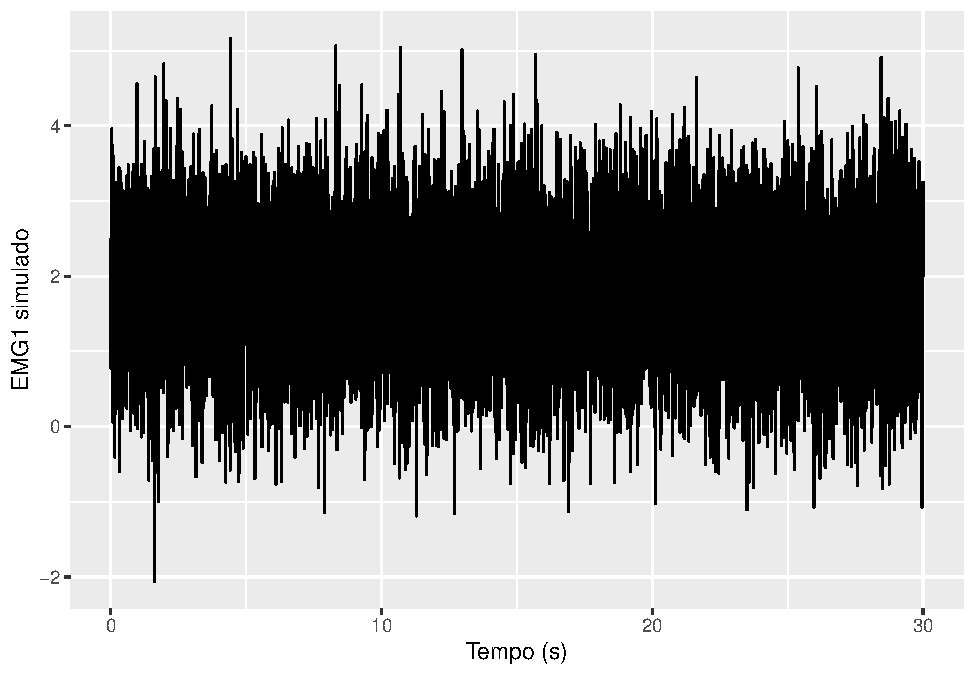
\includegraphics{Modulo4_files/figure-latex/unnamed-chunk-2-1.pdf}

\begin{quote}
Estimar o sinal EMG3 = EMG1 + EMG2, amostrado na mesma frequência de
amostragem que EMG1. Deve-se plotar o gráfico mostrando o sinal gerado
\end{quote}

\begin{Shaded}
\begin{Highlighting}[]
\NormalTok{TempoC }\OtherTok{\textless{}{-}}\NormalTok{ t2}

\NormalTok{AmplitudeC }\OtherTok{\textless{}{-}}\NormalTok{ amplitudes\_EMG2}

\NormalTok{tempo\_discreto\_desejado }\OtherTok{\textless{}{-}}\NormalTok{ t}

\CommentTok{\# Criacao do DataFrame contendo a interpolação}
\NormalTok{df\_c }\OtherTok{\textless{}{-}} \FunctionTok{data.frame}\NormalTok{(}\FunctionTok{spline}\NormalTok{(}\AttributeTok{x =}\NormalTok{ TempoC,}
                        \AttributeTok{y =}\NormalTok{ AmplitudeC,}
                        \AttributeTok{xout =}\NormalTok{ tempo\_discreto\_desejado))}

\NormalTok{amplitude\_interpolado }\OtherTok{\textless{}{-}}\NormalTok{ df\_c}\SpecialCharTok{$}\NormalTok{y}
\NormalTok{tempo\_do\_sinal\_interpolado }\OtherTok{\textless{}{-}}\NormalTok{ df\_c}\SpecialCharTok{$}\NormalTok{x}

\CommentTok{\# Calcula as amplitudes do EMG3}
\NormalTok{amplitudes\_EMG3 }\OtherTok{\textless{}{-}}\NormalTok{ amplitudes\_EMG1 }\SpecialCharTok{+}\NormalTok{ amplitude\_interpolado}

\CommentTok{\# Criando o DataFrame para o EMG3}
\NormalTok{df\_EMG3 }\OtherTok{\textless{}{-}} \FunctionTok{data.frame}\NormalTok{(}\AttributeTok{Amplitudes =}\NormalTok{ amplitudes\_EMG3, }\AttributeTok{t =}\NormalTok{ t)}

\CommentTok{\# Cria o ggplot para o EMG3}
\NormalTok{ggplot3 }\OtherTok{\textless{}{-}}\NormalTok{ ggplot2}\SpecialCharTok{::}\FunctionTok{ggplot}\NormalTok{(df\_EMG3, }\FunctionTok{aes}\NormalTok{ (}\AttributeTok{x =}\NormalTok{ t, }\AttributeTok{y =}\NormalTok{ Amplitudes)) }\SpecialCharTok{+}
  \FunctionTok{geom\_line}\NormalTok{() }\SpecialCharTok{+} \FunctionTok{xlab}\NormalTok{(}\StringTok{"Tempo (s)"}\NormalTok{) }\SpecialCharTok{+}
  \FunctionTok{ylab}\NormalTok{(}\StringTok{"EMG3 simulado"}\NormalTok{)}

\CommentTok{\# Plota o grafico utilizando o ggplot}
\NormalTok{ggplot3}
\end{Highlighting}
\end{Shaded}

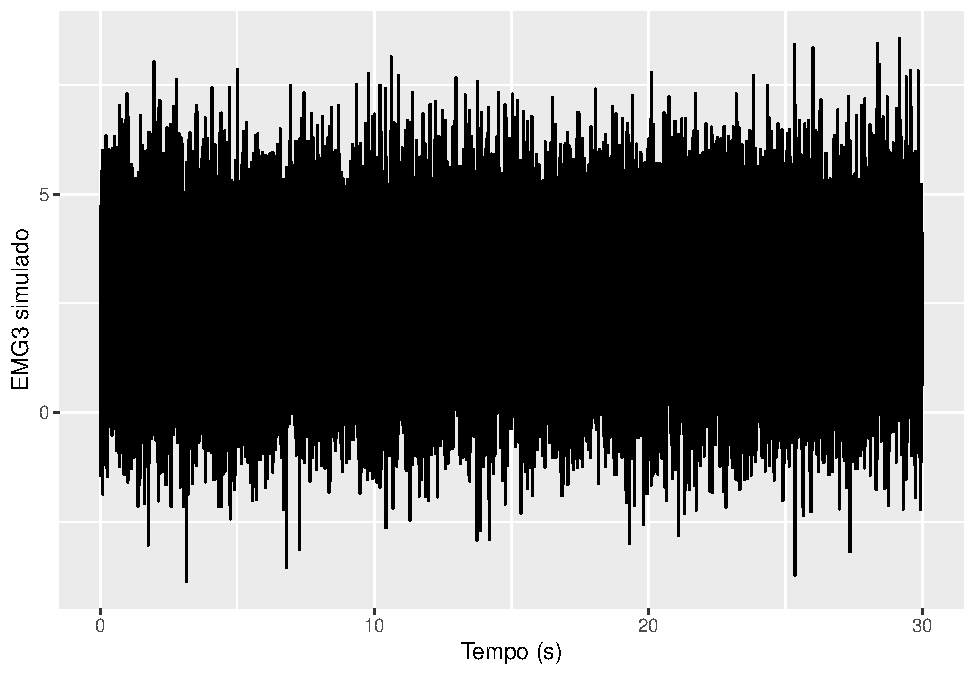
\includegraphics{Modulo4_files/figure-latex/unnamed-chunk-3-1.pdf}

\begin{quote}
Gerar o boxplot, histograma e gráfico da densidade de cada um dos
sinais, EMG1, EMG2 e EMG3. Os resultados devem gerar uma única imagem,
contendo um painel dividido em três linhas e três colunas. A coluna 1
deve ser destinada ao boxplot, a dois ao histograma e a três à
densidade.
\end{quote}

\begin{Shaded}
\begin{Highlighting}[]
\FunctionTok{library}\NormalTok{(patchwork)}

\CommentTok{\# Boxplot EMG1}
\NormalTok{boxplot\_EMG1 }\OtherTok{\textless{}{-}} \FunctionTok{ggplot}\NormalTok{(df\_EMG1, }\FunctionTok{aes}\NormalTok{(}\AttributeTok{x =} \FunctionTok{factor}\NormalTok{(}\StringTok{"EMG1"}\NormalTok{), }\AttributeTok{y =}\NormalTok{ Amplitudes)) }\SpecialCharTok{+}
  \FunctionTok{geom\_boxplot}\NormalTok{() }\SpecialCharTok{+}
  \FunctionTok{labs}\NormalTok{(}\AttributeTok{x =} \StringTok{""}\NormalTok{, }\AttributeTok{y =} \StringTok{"Amplitude"}\NormalTok{) }

\CommentTok{\# Histograma EMG1}
\NormalTok{histograma\_EMG1 }\OtherTok{\textless{}{-}} \FunctionTok{ggplot}\NormalTok{(df\_EMG1, }\FunctionTok{aes}\NormalTok{(}\AttributeTok{x =}\NormalTok{ Amplitudes)) }\SpecialCharTok{+}
  \FunctionTok{geom\_histogram}\NormalTok{(}\AttributeTok{binwidth =} \FloatTok{0.5}\NormalTok{, }\AttributeTok{fill =} \StringTok{"orange"}\NormalTok{, }\AttributeTok{color =} \StringTok{"black"}\NormalTok{) }\SpecialCharTok{+}
  \FunctionTok{labs}\NormalTok{(}\AttributeTok{title =} \StringTok{"EMG1"}\NormalTok{, }\AttributeTok{x =} \StringTok{"Amplitude"}\NormalTok{, }\AttributeTok{y =} \StringTok{"Frequencia"}\NormalTok{) }

\CommentTok{\# Densidade EMG1}
\NormalTok{densidade\_EMG1 }\OtherTok{\textless{}{-}} \FunctionTok{ggplot}\NormalTok{(df\_EMG1, }\FunctionTok{aes}\NormalTok{(}\AttributeTok{x =}\NormalTok{ Amplitudes)) }\SpecialCharTok{+}
  \FunctionTok{geom\_density}\NormalTok{(}\AttributeTok{fill =} \StringTok{"orange"}\NormalTok{, }\AttributeTok{color =} \StringTok{"black"}\NormalTok{) }\SpecialCharTok{+}
  \FunctionTok{labs}\NormalTok{(}\AttributeTok{title =} \StringTok{"EMG1"}\NormalTok{, }\AttributeTok{x =} \StringTok{"Amplitude"}\NormalTok{, }\AttributeTok{y =} \StringTok{"Densidade"}\NormalTok{)}

\CommentTok{\# Boxplot EMG2}
\NormalTok{boxplot\_EMG2 }\OtherTok{\textless{}{-}} \FunctionTok{ggplot}\NormalTok{(df\_EMG2, }\FunctionTok{aes}\NormalTok{(}\AttributeTok{x =} \FunctionTok{factor}\NormalTok{(}\StringTok{"EMG2"}\NormalTok{), }\AttributeTok{y =}\NormalTok{ Amplitudes)) }\SpecialCharTok{+}
  \FunctionTok{geom\_boxplot}\NormalTok{() }\SpecialCharTok{+}
  \FunctionTok{labs}\NormalTok{(}\AttributeTok{x =} \StringTok{""}\NormalTok{, }\AttributeTok{y =} \StringTok{"Amplitude"}\NormalTok{) }

\CommentTok{\# Histograma EMG2}
\NormalTok{histograma\_EMG2 }\OtherTok{\textless{}{-}} \FunctionTok{ggplot}\NormalTok{(df\_EMG2, }\FunctionTok{aes}\NormalTok{(}\AttributeTok{x =}\NormalTok{ Amplitudes)) }\SpecialCharTok{+}
  \FunctionTok{geom\_histogram}\NormalTok{(}\AttributeTok{binwidth =} \FloatTok{0.5}\NormalTok{, }\AttributeTok{fill =} \StringTok{"red"}\NormalTok{, }\AttributeTok{color =} \StringTok{"black"}\NormalTok{) }\SpecialCharTok{+}
  \FunctionTok{labs}\NormalTok{(}\AttributeTok{title =} \StringTok{"EMG2"}\NormalTok{, }\AttributeTok{x =} \StringTok{"Amplitude"}\NormalTok{, }\AttributeTok{y =} \StringTok{"Frequencia"}\NormalTok{) }

\CommentTok{\# Densidade EMG2}
\NormalTok{densidade\_EMG2 }\OtherTok{\textless{}{-}} \FunctionTok{ggplot}\NormalTok{(df\_EMG2, }\FunctionTok{aes}\NormalTok{(}\AttributeTok{x =}\NormalTok{ Amplitudes)) }\SpecialCharTok{+}
  \FunctionTok{geom\_density}\NormalTok{(}\AttributeTok{fill =} \StringTok{"red"}\NormalTok{, }\AttributeTok{color =} \StringTok{"black"}\NormalTok{) }\SpecialCharTok{+}
  \FunctionTok{labs}\NormalTok{(}\AttributeTok{title =} \StringTok{"EMG2"}\NormalTok{, }\AttributeTok{x =} \StringTok{"Amplitude"}\NormalTok{, }\AttributeTok{y =} \StringTok{"Densidade"}\NormalTok{)}

\CommentTok{\# Boxplot EMG3}
\NormalTok{boxplot\_EMG3 }\OtherTok{\textless{}{-}} \FunctionTok{ggplot}\NormalTok{(df\_EMG3, }\FunctionTok{aes}\NormalTok{(}\AttributeTok{x =} \FunctionTok{factor}\NormalTok{(}\StringTok{"EMG3"}\NormalTok{), }\AttributeTok{y =}\NormalTok{ Amplitudes)) }\SpecialCharTok{+}
  \FunctionTok{geom\_boxplot}\NormalTok{() }\SpecialCharTok{+}
  \FunctionTok{labs}\NormalTok{(}\AttributeTok{x =} \StringTok{""}\NormalTok{, }\AttributeTok{y =} \StringTok{"Amplitude"}\NormalTok{) }

\CommentTok{\# Histograma EMG3}
\NormalTok{histograma\_EMG3 }\OtherTok{\textless{}{-}} \FunctionTok{ggplot}\NormalTok{(df\_EMG3, }\FunctionTok{aes}\NormalTok{(}\AttributeTok{x =}\NormalTok{ Amplitudes)) }\SpecialCharTok{+}
  \FunctionTok{geom\_histogram}\NormalTok{(}\AttributeTok{binwidth =} \FloatTok{0.5}\NormalTok{, }\AttributeTok{fill =} \StringTok{"green"}\NormalTok{, }\AttributeTok{color =} \StringTok{"black"}\NormalTok{) }\SpecialCharTok{+}
  \FunctionTok{labs}\NormalTok{(}\AttributeTok{title =} \StringTok{"EMG3"}\NormalTok{, }\AttributeTok{x =} \StringTok{"Amplitude"}\NormalTok{, }\AttributeTok{y =} \StringTok{"Frequencia"}\NormalTok{)}

\CommentTok{\# Densidade EMG3}
\NormalTok{densidade\_EMG3 }\OtherTok{\textless{}{-}} \FunctionTok{ggplot}\NormalTok{(df\_EMG3, }\FunctionTok{aes}\NormalTok{(}\AttributeTok{x =}\NormalTok{ Amplitudes)) }\SpecialCharTok{+}
  \FunctionTok{geom\_density}\NormalTok{(}\AttributeTok{fill =} \StringTok{"green"}\NormalTok{, }\AttributeTok{color =} \StringTok{"black"}\NormalTok{) }\SpecialCharTok{+}
  \FunctionTok{labs}\NormalTok{(}\AttributeTok{title =} \StringTok{"EMG3"}\NormalTok{, }\AttributeTok{x =} \StringTok{"Amplitude"}\NormalTok{, }\AttributeTok{y =} \StringTok{"Densidade"}\NormalTok{)}

\CommentTok{\# Mostrando a tabela }
\NormalTok{(boxplot\_EMG1 }\SpecialCharTok{|}\NormalTok{ histograma\_EMG1 }\SpecialCharTok{|}\NormalTok{ densidade\_EMG1) }\SpecialCharTok{/}
\NormalTok{(boxplot\_EMG2 }\SpecialCharTok{|}\NormalTok{ histograma\_EMG2 }\SpecialCharTok{|}\NormalTok{ densidade\_EMG2) }\SpecialCharTok{/}
\NormalTok{(boxplot\_EMG3 }\SpecialCharTok{|}\NormalTok{ histograma\_EMG3 }\SpecialCharTok{|}\NormalTok{ densidade\_EMG3)}
\end{Highlighting}
\end{Shaded}

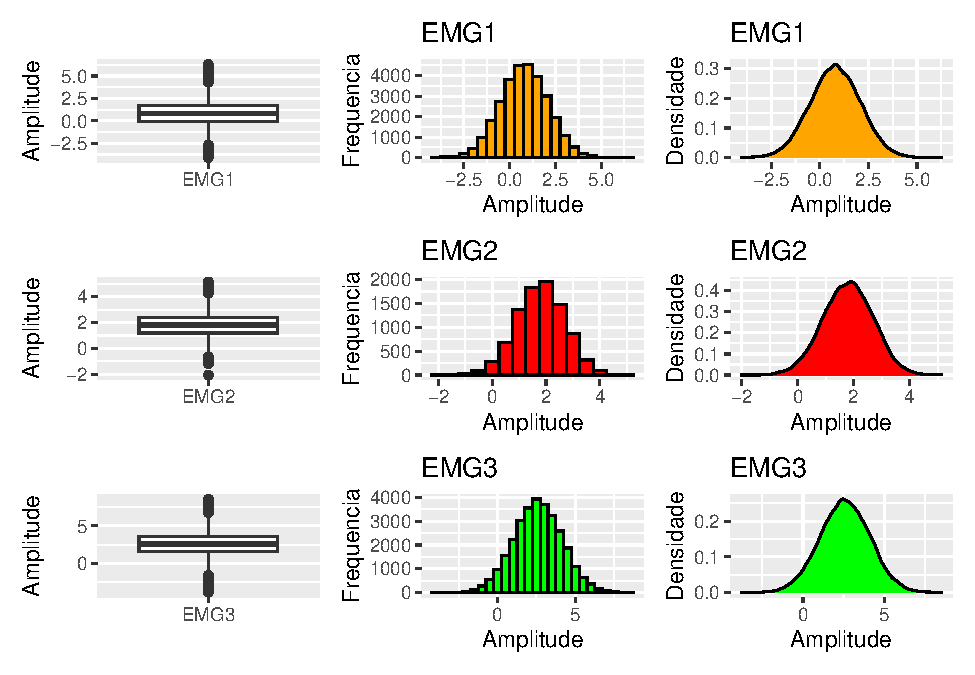
\includegraphics{Modulo4_files/figure-latex/unnamed-chunk-4-1.pdf}

\begin{quote}
Calcular a média, desvio padrão, variância, coeficiente de assimetria e
curtose dos sinais EMG1, EMG2 e EMG3. Os resultados devem ser
apresentados com três casas decimais.
\end{quote}

\begin{Shaded}
\begin{Highlighting}[]
\FunctionTok{library}\NormalTok{(kableExtra)}
\end{Highlighting}
\end{Shaded}

\begin{verbatim}
## Warning: pacote 'kableExtra' foi compilado no R versão 4.4.3
\end{verbatim}

\begin{verbatim}
## 
## Anexando pacote: 'kableExtra'
\end{verbatim}

\begin{verbatim}
## O seguinte objeto é mascarado por 'package:dplyr':
## 
##     group_rows
\end{verbatim}

\begin{Shaded}
\begin{Highlighting}[]
\FunctionTok{library}\NormalTok{(e1071)}
\end{Highlighting}
\end{Shaded}

\begin{verbatim}
## Warning: pacote 'e1071' foi compilado no R versão 4.4.3
\end{verbatim}

\begin{verbatim}
## 
## Anexando pacote: 'e1071'
\end{verbatim}

\begin{verbatim}
## O seguinte objeto é mascarado por 'package:pracma':
## 
##     sigmoid
\end{verbatim}

\begin{Shaded}
\begin{Highlighting}[]
\FunctionTok{library}\NormalTok{(dplyr)}

\CommentTok{\# Calculando a media com a funcao mean()}
\NormalTok{media\_EMG1 }\OtherTok{\textless{}{-}} \FunctionTok{mean}\NormalTok{(df\_EMG1}\SpecialCharTok{$}\NormalTok{Amplitudes)}
\NormalTok{media\_EMG2 }\OtherTok{\textless{}{-}} \FunctionTok{mean}\NormalTok{(df\_EMG2}\SpecialCharTok{$}\NormalTok{Amplitudes)}
\NormalTok{media\_EMG3 }\OtherTok{\textless{}{-}} \FunctionTok{mean}\NormalTok{(df\_EMG3}\SpecialCharTok{$}\NormalTok{Amplitudes)}

\CommentTok{\# Arredondando o resultado para 3 casas decimais}

\NormalTok{media\_EMG1\_3 }\OtherTok{\textless{}{-}} \FunctionTok{round}\NormalTok{(media\_EMG1, }\DecValTok{3}\NormalTok{)}
\NormalTok{media\_EMG2\_3 }\OtherTok{\textless{}{-}} \FunctionTok{round}\NormalTok{(media\_EMG2, }\DecValTok{3}\NormalTok{)}
\NormalTok{media\_EMG3\_3 }\OtherTok{\textless{}{-}} \FunctionTok{round}\NormalTok{(media\_EMG3, }\DecValTok{3}\NormalTok{)}

\CommentTok{\# Calculando o desvio padrao}
\NormalTok{dp\_EMG1 }\OtherTok{\textless{}{-}} \FunctionTok{sd}\NormalTok{(df\_EMG1}\SpecialCharTok{$}\NormalTok{Amplitudes)}
\NormalTok{dp\_EMG2 }\OtherTok{\textless{}{-}} \FunctionTok{sd}\NormalTok{(df\_EMG2}\SpecialCharTok{$}\NormalTok{Amplitudes)}
\NormalTok{dp\_EMG3 }\OtherTok{\textless{}{-}} \FunctionTok{sd}\NormalTok{(df\_EMG3}\SpecialCharTok{$}\NormalTok{Amplitudes)}

\CommentTok{\# Arrendondando o resultado para 3 casas decimais}
\NormalTok{dp\_EMG1\_3 }\OtherTok{\textless{}{-}} \FunctionTok{round}\NormalTok{(dp\_EMG1, }\DecValTok{3}\NormalTok{)}
\NormalTok{dp\_EMG2\_3 }\OtherTok{\textless{}{-}} \FunctionTok{round}\NormalTok{(dp\_EMG2, }\DecValTok{3}\NormalTok{)}
\NormalTok{dp\_EMG3\_3 }\OtherTok{\textless{}{-}} \FunctionTok{round}\NormalTok{(dp\_EMG3, }\DecValTok{3}\NormalTok{)}

\CommentTok{\# Calculando a variancia}
\NormalTok{v\_EMG1 }\OtherTok{\textless{}{-}} \FunctionTok{var}\NormalTok{(df\_EMG1}\SpecialCharTok{$}\NormalTok{Amplitudes)}
\NormalTok{v\_EMG2 }\OtherTok{\textless{}{-}} \FunctionTok{var}\NormalTok{(df\_EMG2}\SpecialCharTok{$}\NormalTok{Amplitudes)}
\NormalTok{v\_EMG3 }\OtherTok{\textless{}{-}} \FunctionTok{var}\NormalTok{(df\_EMG3}\SpecialCharTok{$}\NormalTok{Amplitudes)}

\CommentTok{\# Arredondando resultado para 3 casas decimais}
\NormalTok{v\_EMG1\_3 }\OtherTok{\textless{}{-}} \FunctionTok{round}\NormalTok{(v\_EMG1, }\DecValTok{3}\NormalTok{)}
\NormalTok{v\_EMG2\_3 }\OtherTok{\textless{}{-}} \FunctionTok{round}\NormalTok{(v\_EMG2, }\DecValTok{3}\NormalTok{)}
\NormalTok{v\_EMG3\_3 }\OtherTok{\textless{}{-}} \FunctionTok{round}\NormalTok{(v\_EMG3, }\DecValTok{3}\NormalTok{)}

\CommentTok{\# Calculando o coeficiente de assimetria }
\NormalTok{coefassim\_EMG1 }\OtherTok{\textless{}{-}} \FunctionTok{skewness}\NormalTok{(df\_EMG1}\SpecialCharTok{$}\NormalTok{Amplitudes)}
\NormalTok{coefassim\_EMG2 }\OtherTok{\textless{}{-}} \FunctionTok{skewness}\NormalTok{(df\_EMG2}\SpecialCharTok{$}\NormalTok{Amplitudes)}
\NormalTok{coefassim\_EMG3 }\OtherTok{\textless{}{-}} \FunctionTok{skewness}\NormalTok{(df\_EMG3}\SpecialCharTok{$}\NormalTok{Amplitudes)}

\CommentTok{\# Arredondando resultado para 3 casas decimais}
\NormalTok{coefassim\_EMG1\_3 }\OtherTok{\textless{}{-}} \FunctionTok{round}\NormalTok{(coefassim\_EMG1, }\DecValTok{3}\NormalTok{)}
\NormalTok{coefassim\_EMG2\_3 }\OtherTok{\textless{}{-}} \FunctionTok{round}\NormalTok{(coefassim\_EMG2, }\DecValTok{3}\NormalTok{)}
\NormalTok{coefassim\_EMG3\_3 }\OtherTok{\textless{}{-}} \FunctionTok{round}\NormalTok{(coefassim\_EMG3, }\DecValTok{3}\NormalTok{)}

\CommentTok{\# Calculando o curtose}
\NormalTok{curt\_EMG1 }\OtherTok{\textless{}{-}} \FunctionTok{kurtosis}\NormalTok{(df\_EMG1}\SpecialCharTok{$}\NormalTok{Amplitudes)}
\NormalTok{curt\_EMG2 }\OtherTok{\textless{}{-}} \FunctionTok{kurtosis}\NormalTok{(df\_EMG2}\SpecialCharTok{$}\NormalTok{Amplitudes)}
\NormalTok{curt\_EMG3 }\OtherTok{\textless{}{-}} \FunctionTok{kurtosis}\NormalTok{(df\_EMG3}\SpecialCharTok{$}\NormalTok{Amplitudes)}

\CommentTok{\# Arredondando resultado para 3 casas decimais}
\NormalTok{curt\_EMG1\_3 }\OtherTok{\textless{}{-}} \FunctionTok{round}\NormalTok{(curt\_EMG1, }\DecValTok{3}\NormalTok{)}
\NormalTok{curt\_EMG2\_3 }\OtherTok{\textless{}{-}} \FunctionTok{round}\NormalTok{(curt\_EMG2, }\DecValTok{3}\NormalTok{)}
\NormalTok{curt\_EMG3\_3 }\OtherTok{\textless{}{-}} \FunctionTok{round}\NormalTok{(curt\_EMG3, }\DecValTok{3}\NormalTok{)}

\CommentTok{\# Criando um dataframe}

\NormalTok{df }\OtherTok{\textless{}{-}} \FunctionTok{data.frame}\NormalTok{( }\AttributeTok{sinais =} \FunctionTok{c}\NormalTok{(}\StringTok{"EMG1"}\NormalTok{, }\StringTok{"EMG2"}\NormalTok{, }\StringTok{"EMG3"}\NormalTok{),}
                  \AttributeTok{mean =} \FunctionTok{c}\NormalTok{(media\_EMG1\_3, media\_EMG2\_3, media\_EMG3\_3),}
                  \AttributeTok{dp =} \FunctionTok{c}\NormalTok{(dp\_EMG1\_3, dp\_EMG2\_3, dp\_EMG3\_3),}
                  \AttributeTok{var =} \FunctionTok{c}\NormalTok{(v\_EMG1\_3, v\_EMG2\_3, v\_EMG3\_3),}
                  \AttributeTok{ca =} \FunctionTok{c}\NormalTok{(coefassim\_EMG1\_3, coefassim\_EMG2\_3, coefassim\_EMG3\_3),}
                  \AttributeTok{curtose =} \FunctionTok{c}\NormalTok{(curt\_EMG1\_3, curt\_EMG2\_3, curt\_EMG3\_3))}

\NormalTok{df }\SpecialCharTok{\%\textgreater{}\%} \FunctionTok{kbl}\NormalTok{() }\SpecialCharTok{\%\textgreater{}\%} \FunctionTok{kable\_styling}\NormalTok{()}
\end{Highlighting}
\end{Shaded}

\begin{table}
\centering
\begin{tabular}[t]{l|r|r|r|r|r}
\hline
sinais & mean & dp & var & ca & curtose\\
\hline
EMG1 & 0.793 & 1.295 & 1.676 & -0.020 & 0.012\\
\hline
EMG2 & 1.794 & 0.893 & 0.797 & -0.038 & 0.011\\
\hline
EMG3 & 2.587 & 1.535 & 2.357 & -0.015 & 0.001\\
\hline
\end{tabular}
\end{table}

\newpage
\section*{Questão 2}

\begin{quote}
Considerando o conceito de precisão e acurácia disponível, você deverá:
\end{quote}

\begin{quote}
Propor uma questão que simule a geração de sinais com (i) alta precisão
e alta exatidão, (ii) baixa precisão e alta exatidão, (iii) alta
precisão e baixa exatidão e (iv) baixa precisão e baixa exatidão.
\end{quote}

Suponha que você seja um pesquisador monitorando a temperatura dentro de
uma estufa agrícola. Para garantir o crescimento ideal das plantas, a
temperatura deve ser mantida em torno de 25°C. Você coletará dados de
temperatura em quatro cenários distintos:

\begin{enumerate}
\def\labelenumi{\arabic{enumi}.}
\item
  Alta precisão e alta exatidão: A temperatura varia pouco em torno do
  valor desejado, por exemplo, distribuição normal com média de 25°C e
  desvio padrão de 0,5°C.
\item
  Baixa precisão e alta exatidão: A temperatura varia bastante, mas
  ainda mantém a média em torno do valor ideal, por exemplo,
  distribuição uniforme entre 22°C e 28°C.
\item
  Alta precisão e baixa exatidão: A temperatura se mantém estável, mas
  abaixo do ideal, por exemplo, distribuição normal com média de 23°C e
  desvio padrão de 0,5°C.
\item
  Baixa precisão e baixa exatidão: A temperatura varia muito e não se
  concentra no valor desejado, por exemplo, distribuição uniforme entre
  20°C e 30°C.
\end{enumerate}

\begin{quote}
Desenvolver um programa em R que solucione o problema proposto. Os
sinais gerados devem ser plotados em uma única imagem, dividida em uma
coluna e quatro linhas. Deve-se incluir unidades e legenda para cada
gráfico.
\end{quote}

\begin{Shaded}
\begin{Highlighting}[]
\FunctionTok{library}\NormalTok{(tidyverse)}

\CommentTok{\# Amplitudes do Sinal (1) {-} Alta precisão e alta exatidão}
\NormalTok{temp1 }\OtherTok{\textless{}{-}} \FunctionTok{rnorm}\NormalTok{(}\DecValTok{1000}\NormalTok{, }\AttributeTok{mean =} \DecValTok{25}\NormalTok{, }\AttributeTok{sd =} \FloatTok{0.5}\NormalTok{)}
\NormalTok{temp1 }\OtherTok{\textless{}{-}} \FunctionTok{pmax}\NormalTok{(}\FunctionTok{pmin}\NormalTok{(temp1, }\DecValTok{30}\NormalTok{), }\DecValTok{20}\NormalTok{)}

\CommentTok{\# Amplitudes do Sinal (2) {-} Baixa precisão e alta exatidão}
\NormalTok{temp2 }\OtherTok{\textless{}{-}} \FunctionTok{runif}\NormalTok{(}\DecValTok{1000}\NormalTok{, }\AttributeTok{min =} \DecValTok{22}\NormalTok{, }\AttributeTok{max =} \DecValTok{28}\NormalTok{)}
\NormalTok{temp2 }\OtherTok{\textless{}{-}} \FunctionTok{pmax}\NormalTok{(}\FunctionTok{pmin}\NormalTok{(temp2, }\DecValTok{30}\NormalTok{), }\DecValTok{20}\NormalTok{)}

\CommentTok{\# Amplitudes do Sinal (3) {-} Alta precisão e baixa exatidão}
\NormalTok{temp3 }\OtherTok{\textless{}{-}} \FunctionTok{rnorm}\NormalTok{(}\DecValTok{1000}\NormalTok{, }\AttributeTok{mean =} \DecValTok{23}\NormalTok{, }\AttributeTok{sd =} \FloatTok{0.5}\NormalTok{)}
\NormalTok{temp3 }\OtherTok{\textless{}{-}} \FunctionTok{pmax}\NormalTok{(}\FunctionTok{pmin}\NormalTok{(temp3, }\DecValTok{30}\NormalTok{), }\DecValTok{20}\NormalTok{)}

\CommentTok{\# Amplitudes do Sinal (4) {-} Baixa precisão e baixa exatidão}
\NormalTok{temp4 }\OtherTok{\textless{}{-}} \FunctionTok{runif}\NormalTok{(}\DecValTok{1000}\NormalTok{, }\AttributeTok{min =} \DecValTok{20}\NormalTok{, }\AttributeTok{max =} \DecValTok{30}\NormalTok{)}
\NormalTok{temp4 }\OtherTok{\textless{}{-}} \FunctionTok{pmax}\NormalTok{(}\FunctionTok{pmin}\NormalTok{(temp4, }\DecValTok{30}\NormalTok{), }\DecValTok{20}\NormalTok{)}

\CommentTok{\# Criando vetor de tempo}
\NormalTok{t }\OtherTok{\textless{}{-}} \FunctionTok{rep}\NormalTok{(}\DecValTok{1}\SpecialCharTok{:}\DecValTok{1000}\NormalTok{, }\DecValTok{4}\NormalTok{)}

\CommentTok{\# Criando data frames para os sinais}
\NormalTok{df1 }\OtherTok{\textless{}{-}} \FunctionTok{data.frame}\NormalTok{(}\AttributeTok{temperatura =}\NormalTok{ temp1, }\AttributeTok{t =}\NormalTok{ t, }\AttributeTok{group =} \StringTok{\textquotesingle{}Alta precisão e alta exatidão\textquotesingle{}}\NormalTok{)}
\NormalTok{df2 }\OtherTok{\textless{}{-}} \FunctionTok{data.frame}\NormalTok{(}\AttributeTok{temperatura =}\NormalTok{ temp2, }\AttributeTok{t =}\NormalTok{ t, }\AttributeTok{group =} \StringTok{\textquotesingle{}Baixa precisão e alta exatidão\textquotesingle{}}\NormalTok{)}
\NormalTok{df3 }\OtherTok{\textless{}{-}} \FunctionTok{data.frame}\NormalTok{(}\AttributeTok{temperatura =}\NormalTok{ temp3, }\AttributeTok{t =}\NormalTok{ t, }\AttributeTok{group =} \StringTok{\textquotesingle{}Alta precisão e baixa exatidão\textquotesingle{}}\NormalTok{)}
\NormalTok{df4 }\OtherTok{\textless{}{-}} \FunctionTok{data.frame}\NormalTok{(}\AttributeTok{temperatura =}\NormalTok{ temp4, }\AttributeTok{t =}\NormalTok{ t, }\AttributeTok{group =} \StringTok{\textquotesingle{}Baixa precisão e baixa exatidão\textquotesingle{}}\NormalTok{)}

\CommentTok{\# Unindo os data frames}
\NormalTok{df }\OtherTok{\textless{}{-}} \FunctionTok{rbind}\NormalTok{(df1, df2, df3, df4)}

\CommentTok{\# Plotando os sinais ao longo do tempo}
\FunctionTok{ggplot}\NormalTok{(df, }\FunctionTok{aes}\NormalTok{(}\AttributeTok{x =}\NormalTok{ t, }\AttributeTok{y =}\NormalTok{ temperatura, }\AttributeTok{color =}\NormalTok{ group)) }\SpecialCharTok{+}
  \FunctionTok{geom\_line}\NormalTok{() }\SpecialCharTok{+}
  \FunctionTok{scale\_color\_manual}\NormalTok{(}\AttributeTok{values =} \FunctionTok{c}\NormalTok{(}\StringTok{"red"}\NormalTok{, }\StringTok{"blue"}\NormalTok{, }\StringTok{"green"}\NormalTok{, }\StringTok{"purple"}\NormalTok{)) }\SpecialCharTok{+}
  \FunctionTok{facet\_wrap}\NormalTok{(}\SpecialCharTok{\textasciitilde{}}\NormalTok{ group, }\AttributeTok{ncol =} \DecValTok{1}\NormalTok{, }\AttributeTok{scales =} \StringTok{"free\_y"}\NormalTok{) }\SpecialCharTok{+}
  \FunctionTok{xlab}\NormalTok{(}\StringTok{"Tempo"}\NormalTok{) }\SpecialCharTok{+}
  \FunctionTok{ylab}\NormalTok{(}\StringTok{"Temperatura (°C)"}\NormalTok{) }\SpecialCharTok{+}
  \FunctionTok{theme\_minimal}\NormalTok{()}
\end{Highlighting}
\end{Shaded}

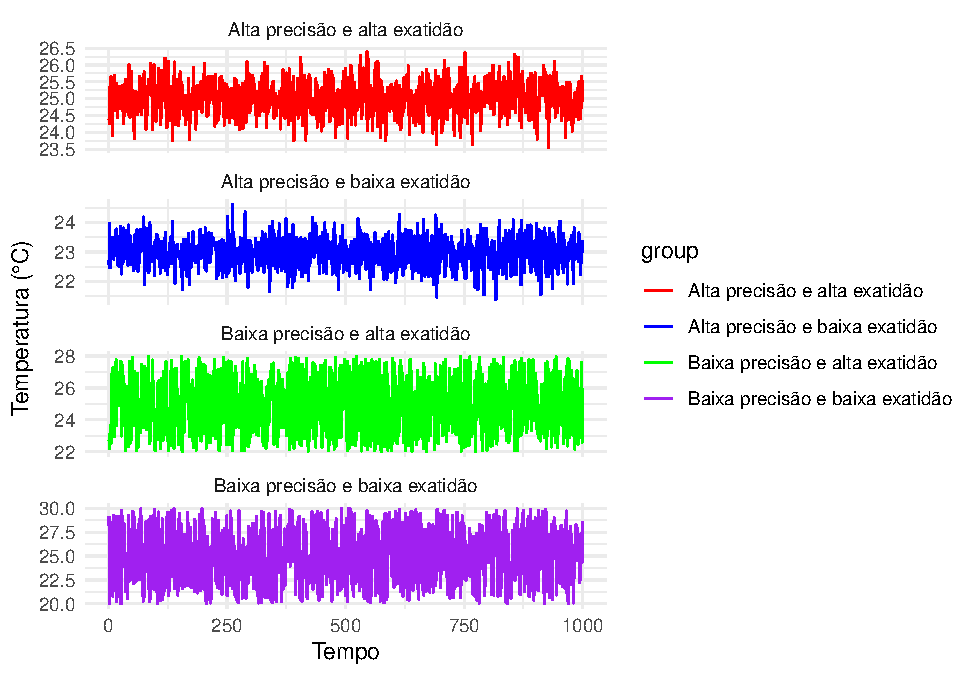
\includegraphics{Modulo4_files/figure-latex/unnamed-chunk-6-1.pdf}

\begin{quote}
Plota um gráfico, usando o ggplot, reportando os resultados como
exemplificado na Figura 1
\end{quote}

\begin{Shaded}
\begin{Highlighting}[]
\CommentTok{\# Plotando as distribuições das temperaturas}
\FunctionTok{ggplot}\NormalTok{(df, }\FunctionTok{aes}\NormalTok{(}\AttributeTok{x =}\NormalTok{ temperatura, }\AttributeTok{fill =}\NormalTok{ group)) }\SpecialCharTok{+}
  \FunctionTok{geom\_density}\NormalTok{(}\AttributeTok{alpha =} \FloatTok{0.5}\NormalTok{) }\SpecialCharTok{+}
  \FunctionTok{scale\_fill\_manual}\NormalTok{(}\AttributeTok{values =} \FunctionTok{c}\NormalTok{(}\StringTok{"pink"}\NormalTok{, }\StringTok{"orange"}\NormalTok{, }\StringTok{"gray"}\NormalTok{, }\StringTok{"yellow"}\NormalTok{)) }\SpecialCharTok{+}
  \FunctionTok{xlab}\NormalTok{(}\StringTok{"Temperatura (°C)"}\NormalTok{) }\SpecialCharTok{+}
  \FunctionTok{ylab}\NormalTok{(}\StringTok{"Densidade"}\NormalTok{) }\SpecialCharTok{+}
  \FunctionTok{theme\_classic}\NormalTok{()}
\end{Highlighting}
\end{Shaded}

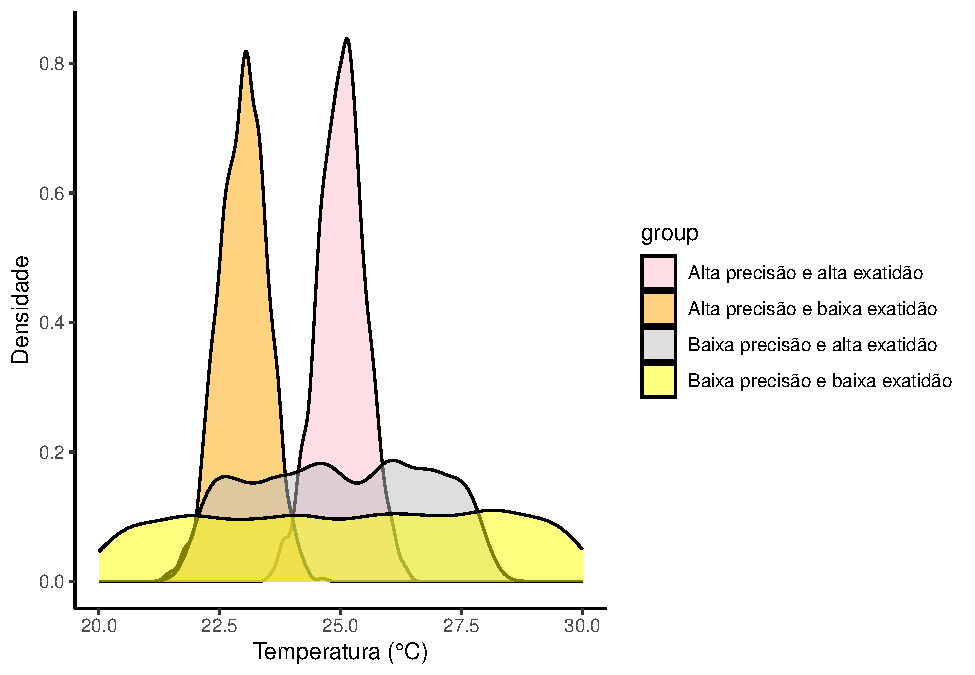
\includegraphics{Modulo4_files/figure-latex/unnamed-chunk-7-1.pdf}

\newpage
\section*{Questão 3}

O conjunto de sinais eletromiográficos, DadosM4-1.txt, disponível na
plataforma moodle, foi originado a partir de uma coleta simultânea de
dados eletromiográficos e inerciais. Os dados foram coletados seguindo o
seguinte protocolo experimental:

\begin{enumerate}
\def\labelenumi{\arabic{enumi}.}
\tightlist
\item
  Os sensores de eletromiografia foram posicionados no músculo tibial
  anterior e nos músculos do tríceps sural. O acelerômetro foi
  posicionado nos dois terços proximais da parte lateral da perna, com o
  eixo y contra a gravidade.
\item
  Com o sujeito na posição ortostática realizou-se o movimento de
  dorsiflexão e flexão plantar. No retorno da flexão realizou-se um
  contato brusco do calcanhar com o solo. 3 Foram realizadas 60
  repetições da tarefa, sem descanso.
\end{enumerate}

Faça a estimativa de parâmetros estatísticos dos sinais
eletromiográficos disponíveis no arquivo DadosM4-1.txt. Os seguintes
passos devem ser executados:

\begin{Shaded}
\begin{Highlighting}[]
\FunctionTok{library}\NormalTok{(dygraphs)}
\FunctionTok{library}\NormalTok{(tidyverse)}

\NormalTok{dadosm4 }\OtherTok{\textless{}{-}} \FunctionTok{read.table}\NormalTok{(}\StringTok{"C:/Users/heito/Desktop/Módulo 4 {-} PSB/DadosM4{-}1.txt"}\NormalTok{, }\AttributeTok{header =} \ConstantTok{FALSE}\NormalTok{, }\AttributeTok{sep =}  \StringTok{" "}\NormalTok{, }\AttributeTok{skip =} \DecValTok{6}\NormalTok{)}

\CommentTok{\# Alterando o nome das variávesi do df}

\FunctionTok{names}\NormalTok{(dadosm4) }\OtherTok{\textless{}{-}} \FunctionTok{c}\NormalTok{(}\StringTok{"AccX"}\NormalTok{, }\StringTok{"AccY"}\NormalTok{, }\StringTok{"MuscAnterior"}\NormalTok{, }\StringTok{"MuscPosterior"}\NormalTok{)}

\CommentTok{\# Criando vetor tempo}

\NormalTok{fs }\OtherTok{\textless{}{-}} \DecValTok{500}

\CommentTok{\# Definindo intervalo entre amostrar}

\NormalTok{dt }\OtherTok{\textless{}{-}} \DecValTok{1}\SpecialCharTok{/}\NormalTok{fs}

\CommentTok{\# Definindo vetor tempo (s)}

\NormalTok{t }\OtherTok{\textless{}{-}} \FunctionTok{seq}\NormalTok{(}\AttributeTok{from=}\DecValTok{0}\NormalTok{, }\AttributeTok{to =}\NormalTok{ dt}\SpecialCharTok{*}\NormalTok{(}\FunctionTok{length}\NormalTok{(dadosm4}\SpecialCharTok{$}\NormalTok{AccY)}\SpecialCharTok{{-}}\DecValTok{1}\NormalTok{), }\AttributeTok{by =}\NormalTok{ dt)}

\NormalTok{dadosm4 }\OtherTok{\textless{}{-}} \FunctionTok{cbind}\NormalTok{(}\AttributeTok{time =}\NormalTok{ t, dadosm4)}

\CommentTok{\# Plotagem do gráfico}

\FunctionTok{dygraph}\NormalTok{(dadosm4[}\FunctionTok{c}\NormalTok{(}\StringTok{"time"}\NormalTok{, }\StringTok{"AccY"}\NormalTok{)], }\AttributeTok{main =} \StringTok{"AccY"}\NormalTok{, }\AttributeTok{group =} \StringTok{"GroupName"}\NormalTok{) }\SpecialCharTok{\%\textgreater{}\%}
  \FunctionTok{dyRangeSelector}\NormalTok{()}
\end{Highlighting}
\end{Shaded}

\begin{Shaded}
\begin{Highlighting}[]
\CommentTok{\# Amplitude Máxima}
\NormalTok{AmpMAX\_AccY }\OtherTok{\textless{}{-}} \FunctionTok{max}\NormalTok{(dadosm4}\SpecialCharTok{$}\NormalTok{AccY) }\SpecialCharTok{{-}} \FunctionTok{min}\NormalTok{(dadosm4}\SpecialCharTok{$}\NormalTok{AccY)}

\NormalTok{lim\_min }\OtherTok{\textless{}{-}} \FloatTok{0.9} \SpecialCharTok{*}\NormalTok{ AmpMAX\_AccY}

\CommentTok{\# Encontrando os picos e armazenando os valores}

\NormalTok{dadosm4 }\OtherTok{\textless{}{-}}\NormalTok{ dadosm4 }\SpecialCharTok{\%\textgreater{}\%}
  \FunctionTok{mutate}\NormalTok{(}\AttributeTok{pico =} \FunctionTok{ifelse}\NormalTok{(dadosm4}\SpecialCharTok{$}\NormalTok{AccY }\SpecialCharTok{{-}} \FunctionTok{min}\NormalTok{(dadosm4}\SpecialCharTok{$}\NormalTok{AccY) }\SpecialCharTok{\textgreater{}=}\NormalTok{ lim\_min, dadosm4}\SpecialCharTok{$}\NormalTok{AccY, }\ConstantTok{NA}\NormalTok{))}
\end{Highlighting}
\end{Shaded}

\begin{quote}
Gere um gráfico ocm os picos encontrados na letra a).
\end{quote}

\begin{Shaded}
\begin{Highlighting}[]
\CommentTok{\# Plotagem do gráfico}
\FunctionTok{ggplot}\NormalTok{(dadosm4, }\FunctionTok{aes}\NormalTok{(}\AttributeTok{x =}\NormalTok{ time, }\AttributeTok{y =}\NormalTok{ pico)) }\SpecialCharTok{+}
  \FunctionTok{geom\_line}\NormalTok{(}\AttributeTok{na.rm =} \ConstantTok{TRUE}\NormalTok{) }\SpecialCharTok{+}
  \FunctionTok{labs}\NormalTok{(}\AttributeTok{title =} \StringTok{"Amplitudes de AccY \textgreater{}= 90\% da Max. Amplitude"}\NormalTok{,}
       \AttributeTok{x =} \StringTok{"Tempo"}\NormalTok{,}
       \AttributeTok{y =} \StringTok{"AccY"}\NormalTok{)}
\end{Highlighting}
\end{Shaded}

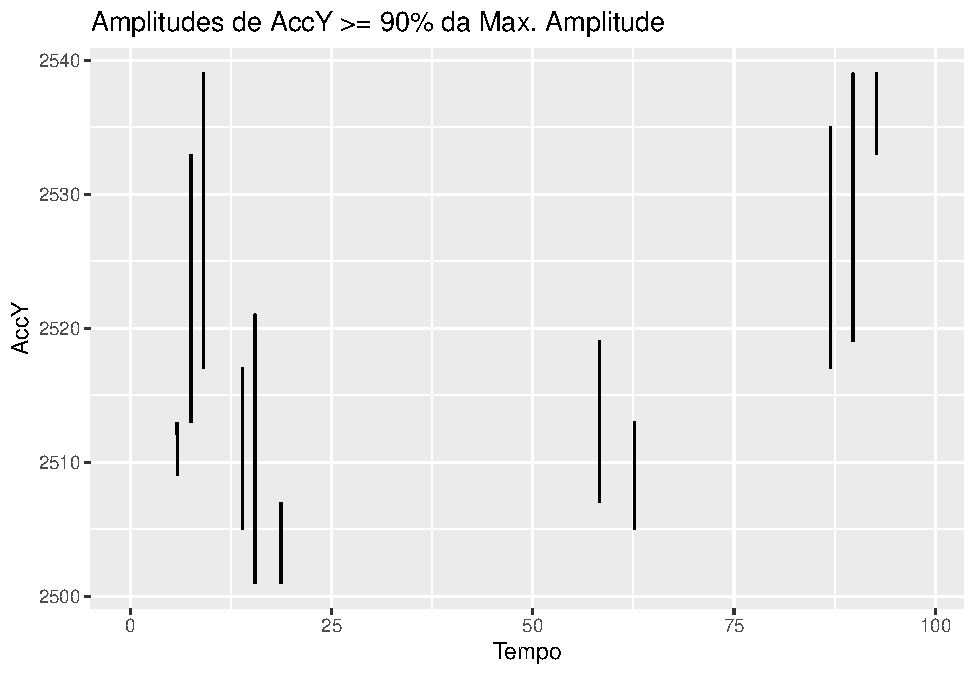
\includegraphics{Modulo4_files/figure-latex/unnamed-chunk-10-1.pdf}

\begin{quote}
Calcule as estatísticas Média, Mediana, Moda, Amplitude, Variância,
Coeficiente de Variação, Distância Interquartil para cada janela de
sinal do músculo tibial anterior. O tamanho da janela deve ser de 500
ms, e o início da mesma deve ser a partir de cada um dos picos
detectados na letra a).
\end{quote}

\begin{Shaded}
\begin{Highlighting}[]
\CommentTok{\# Cálculo dos parâmetros}
\NormalTok{x }\OtherTok{\textless{}{-}}\NormalTok{ dadosm4}\SpecialCharTok{$}\NormalTok{MuscPosterior  }\CommentTok{\# Definição da variável correta}

\CommentTok{\# Tamanho da janela}
\NormalTok{janela }\OtherTok{\textless{}{-}} \DecValTok{500}

\CommentTok{\# Índice dos picos encontrados}
\NormalTok{indice\_picos }\OtherTok{\textless{}{-}} \FunctionTok{which}\NormalTok{(}\SpecialCharTok{!}\FunctionTok{is.na}\NormalTok{(dadosm4}\SpecialCharTok{$}\NormalTok{pico))}

\CommentTok{\# Criando um data frame vazio para armazenar os resultados}
\NormalTok{df }\OtherTok{\textless{}{-}} \FunctionTok{data.frame}\NormalTok{()}

\CommentTok{\# Loop para percorrer os picos}
\ControlFlowTok{for}\NormalTok{ (i }\ControlFlowTok{in}\NormalTok{ indice\_picos)\{}
\NormalTok{  indx1 }\OtherTok{\textless{}{-}}\NormalTok{ i }\SpecialCharTok{{-}} \FunctionTok{floor}\NormalTok{(janela }\SpecialCharTok{/} \DecValTok{2}\NormalTok{)}
\NormalTok{  indx2 }\OtherTok{\textless{}{-}}\NormalTok{ i }\SpecialCharTok{+} \FunctionTok{ceiling}\NormalTok{(janela }\SpecialCharTok{/} \DecValTok{2}\NormalTok{) }\SpecialCharTok{{-}} \DecValTok{1}
  
  \CommentTok{\# Cálculo dos valores desejados}
  \ControlFlowTok{if}\NormalTok{(indx1 }\SpecialCharTok{\textgreater{}} \DecValTok{0} \SpecialCharTok{\&}\NormalTok{ indx2 }\SpecialCharTok{\textless{}=} \FunctionTok{length}\NormalTok{(x)) \{ }
\NormalTok{    media }\OtherTok{\textless{}{-}} \FunctionTok{mean}\NormalTok{(x[indx1}\SpecialCharTok{:}\NormalTok{indx2])}
\NormalTok{    mediana }\OtherTok{\textless{}{-}} \FunctionTok{median}\NormalTok{(x[indx1}\SpecialCharTok{:}\NormalTok{indx2])}
\NormalTok{    moda }\OtherTok{\textless{}{-}} \FunctionTok{as.numeric}\NormalTok{(}\FunctionTok{names}\NormalTok{(}\FunctionTok{table}\NormalTok{(x[indx1}\SpecialCharTok{:}\NormalTok{indx2]))[}\FunctionTok{which.max}\NormalTok{(}\FunctionTok{table}\NormalTok{(x[indx1}\SpecialCharTok{:}\NormalTok{indx2]))])}
\NormalTok{    amplitude }\OtherTok{\textless{}{-}} \FunctionTok{max}\NormalTok{(x[indx1}\SpecialCharTok{:}\NormalTok{indx2]) }\SpecialCharTok{{-}} \FunctionTok{min}\NormalTok{(x[indx1}\SpecialCharTok{:}\NormalTok{indx2])}
\NormalTok{    variancia }\OtherTok{\textless{}{-}} \FunctionTok{var}\NormalTok{(x[indx1}\SpecialCharTok{:}\NormalTok{indx2])}
\NormalTok{    cv }\OtherTok{\textless{}{-}} \FunctionTok{sd}\NormalTok{(x[indx1}\SpecialCharTok{:}\NormalTok{indx2]) }\SpecialCharTok{/} \FunctionTok{mean}\NormalTok{(x[indx1}\SpecialCharTok{:}\NormalTok{indx2])}
\NormalTok{    iqr }\OtherTok{\textless{}{-}} \FunctionTok{IQR}\NormalTok{(x[indx1}\SpecialCharTok{:}\NormalTok{indx2])}
    
    \CommentTok{\# Armazenando os resultados no data frame}
\NormalTok{    df }\OtherTok{\textless{}{-}} \FunctionTok{rbind}\NormalTok{(df, }\FunctionTok{data.frame}\NormalTok{(}\AttributeTok{pico =}\NormalTok{ i, }\AttributeTok{media =}\NormalTok{ media, }\AttributeTok{mediana =}\NormalTok{ mediana, }\AttributeTok{moda =}\NormalTok{ moda,}
                               \AttributeTok{amplitude =}\NormalTok{ amplitude, }\AttributeTok{variancia =}\NormalTok{ variancia, }\AttributeTok{cv =}\NormalTok{ cv, }\AttributeTok{iqr =}\NormalTok{ iqr))}
\NormalTok{  \}}
\NormalTok{\}}

\CommentTok{\# Exibindo o data frame com os resultados}
\NormalTok{df}
\end{Highlighting}
\end{Shaded}

\begin{verbatim}
##     pico    media mediana moda amplitude variancia        cv   iqr
## 1   2910 2066.424    2051 2035      3957 134332.67 0.1773664 136.5
## 2   2911 2068.902    2051 2035      3957 131600.60 0.1753432 138.0
## 3   3768 2068.578    2048 2075      4095 229571.68 0.2316260 159.5
## 4   3769 2070.348    2048 2075      4095 227723.77 0.2304946 159.0
## 5   3770 2070.536    2048 2075      4095 227697.24 0.2304603 159.0
## 6   4552 2064.994    2052 2095      3956 156894.70 0.1918162 173.5
## 7   4553 2063.906    2052 2095      3956 156313.52 0.1915616 172.5
## 8   4554 2065.114    2052 2095      3956 155549.72 0.1909812 172.0
## 9   4555 2063.606    2051 2095      3956 154487.05 0.1904668 170.5
## 10  6950 2073.330    2055 2019      4095 195665.31 0.2133480 192.0
## 11  6951 2072.434    2055 2019      4095 195137.20 0.2131520 190.5
## 12  6952 2071.026    2055 2019      4095 193875.16 0.2126060 190.5
## 13  7742 2072.692    2053 1947      4095 188807.40 0.2096403 180.0
## 14  7743 2070.528    2053 1947      4095 187452.67 0.2091051 179.0
## 15  7744 2067.718    2053 1947      4095 183531.19 0.2071875 177.0
## 16  7745 2071.012    2053 1947      4095 177524.99 0.2034451 176.5
## 17  9362 2055.338    2053 2011      3732 145122.20 0.1853462 164.5
## 18  9363 2054.450    2053 2011      3732 144726.95 0.1851736 162.5
## 19 11714 2061.740    2058 2067      3998 175905.70 0.2034258 180.0
## 20 29131 2034.980    2053 2075      3800 140080.08 0.1839196 194.0
## 21 29132 2033.560    2053 2075      3800 139295.43 0.1835319 194.0
## 22 29133 2036.306    2053 2075      3800 134681.53 0.1802233 194.0
## 23 31331 2052.260    2044 2051      3886 105066.14 0.1579425 138.0
## 24 31332 2049.866    2044 2051      3886 102127.91 0.1559002 136.5
## 25 31333 2047.248    2044 2051      3886  98555.35 0.1533450 136.0
## 26 43466 2057.690    2049 2067      4095 142306.08 0.1833293 124.0
## 27 43467 2055.786    2049 2067      4095 140755.94 0.1824969 123.0
## 28 43468 2054.710    2048 2067      4095 140206.61 0.1822358 122.5
## 29 43469 2055.362    2048 2067      4095 139983.13 0.1820328 122.0
## 30 44883 2055.248    2051 2021      4095 125150.06 0.1721279 129.0
## 31 44884 2053.732    2051 2021      4095 124009.23 0.1714681 128.5
## 32 44885 2053.400    2051 2021      4095 123943.74 0.1714505 128.5
## 33 44886 2054.648    2051 2021      4095 123095.84 0.1707593 128.0
## 34 44887 2055.600    2051 2021      4095 122553.79 0.1703040 126.5
## 35 44888 2059.686    2051 2021      4095 114069.46 0.1639773 126.0
## 36 44889 2058.626    2051 2021      4095 113472.88 0.1636321 124.5
## 37 44890 2057.130    2051 2021      4095 112258.32 0.1628724 122.5
## 38 46328 2057.948    2050 2057      4095 110091.48 0.1612287  98.5
## 39 46329 2058.208    2050 2043      4095 110049.76 0.1611778  98.5
## 40 46330 2059.196    2051 2043      4095 109592.98 0.1607658  97.0
## 41 46331 2060.440    2051 2043      4095 108860.50 0.1601309  96.5
## 42 46332 2061.700    2051 2043      4095 108009.38 0.1594062  95.0
## 43 46333 2061.248    2051 2043      4095 107987.16 0.1594248  96.0
\end{verbatim}

\begin{quote}
Faça um gráfico que descreva a variação da mediana em função do tempo
\end{quote}

\begin{Shaded}
\begin{Highlighting}[]
\CommentTok{\# Seleção do sinal de interesse}
\NormalTok{y }\OtherTok{\textless{}{-}}\NormalTok{ dadosm4}\SpecialCharTok{$}\NormalTok{MuscPosterior  }

\CommentTok{\# Definição do tamanho da janela (número de amostras)}
\NormalTok{Nwnd }\OtherTok{\textless{}{-}} \DecValTok{500}  

\CommentTok{\# Gerando os índices iniciais de cada janela}
\NormalTok{indx1 }\OtherTok{\textless{}{-}} \FunctionTok{seq}\NormalTok{(}\AttributeTok{from =} \DecValTok{1}\NormalTok{, }\AttributeTok{to =} \FunctionTok{length}\NormalTok{(y), }\AttributeTok{by =}\NormalTok{ Nwnd)}
\NormalTok{N }\OtherTok{\textless{}{-}} \FunctionTok{length}\NormalTok{(indx1)  }\CommentTok{\# Número de janelas}

\CommentTok{\# Inicializando um data frame para armazenar os resultados}
\NormalTok{dfenv }\OtherTok{\textless{}{-}} \FunctionTok{data.frame}\NormalTok{(}
  \AttributeTok{time =} \FunctionTok{rep}\NormalTok{(}\ConstantTok{NA}\NormalTok{, }\AttributeTok{times =}\NormalTok{ N }\SpecialCharTok{{-}} \DecValTok{1}\NormalTok{),}
  \AttributeTok{mediana =} \ConstantTok{NA}
\NormalTok{)}

\CommentTok{\# Loop para calcular a mediana em cada janela}
\ControlFlowTok{for}\NormalTok{ (i }\ControlFlowTok{in} \DecValTok{1}\SpecialCharTok{:}\NormalTok{(N }\SpecialCharTok{{-}} \DecValTok{1}\NormalTok{)) \{}
  \CommentTok{\# Calcula o tempo centralizado em cada janela}
\NormalTok{  dfenv}\SpecialCharTok{$}\NormalTok{time[i] }\OtherTok{\textless{}{-}}\NormalTok{ (indx1[i] }\SpecialCharTok{+}\NormalTok{ (indx1[i }\SpecialCharTok{+} \DecValTok{1}\NormalTok{] }\SpecialCharTok{{-}}\NormalTok{ indx1[i]) }\SpecialCharTok{/} \DecValTok{2}\NormalTok{) }\SpecialCharTok{*}\NormalTok{ dt  }
  \CommentTok{\# Calcula a mediana do sinal na janela atual}
\NormalTok{  dfenv}\SpecialCharTok{$}\NormalTok{mediana[i] }\OtherTok{\textless{}{-}} \FunctionTok{median}\NormalTok{(y[indx1[i]}\SpecialCharTok{:}\NormalTok{indx1[i }\SpecialCharTok{+} \DecValTok{1}\NormalTok{]])}
\NormalTok{\}}

\CommentTok{\# Plotando os resultados}
\FunctionTok{dygraph}\NormalTok{(dfenv, }\AttributeTok{main =} \StringTok{"Mediana x Tempo"}\NormalTok{, }\AttributeTok{group =} \StringTok{"GroupName"}\NormalTok{) }\SpecialCharTok{\%\textgreater{}\%} 
  \FunctionTok{dyRangeSelector}\NormalTok{()}
\end{Highlighting}
\end{Shaded}


\end{document}
